\documentclass{article}

%%%%%%%%%%%%%%%%%
%%%%%%%%%% PACKAGES
%%%%%%%%%%%%%%%%%
\usepackage{amsfonts}
\usepackage{amsmath}
\usepackage{amsthm}
\usepackage{amssymb}

\usepackage{blindtext}
\usepackage{enumerate}
\usepackage{fancyhdr}
\usepackage{hyperref}
\usepackage[margin=1.5in]{geometry}
\usepackage{multicol}
\usepackage{parskip}
\usepackage{titlesec}

\usepackage[dvipsnames]{xcolor}
\usepackage{graphicx}
\usepackage{pagecolor}
\usepackage{tcolorbox}

\usepackage{pgf}
\usepackage{tikz}
\usepackage{tkz-berge}
\usetikzlibrary{arrows, automata, backgrounds, petri, topaths, shapes}

%%%%%%%%%%%%%%%%%
%%%%%%%%% TCOLORBOX
%%%%%%%%%%%%%%%%%
\tcbuselibrary{theorems}
\tcbuselibrary{skins}
\usepackage{cleveref}

\tcbset{
defstyle/.style={fonttitle=\bfseries\upshape, fontupper=\slshape,
arc=0mm, colback=blue!5!white,colframe=blue!75!black},
theostyle/.style={fonttitle=\bfseries\upshape, fontupper=\slshape,
colback=red!10!white,colframe=red!75!black},
}

\newtcbtheorem[number within=subsection,crefname={definition}{definitions}]{Definition}{Definition}{defstyle}{def}
\newtcbtheorem[use counter from=Definition,crefname={theorem2}{theorems}]{Theorem}{Theorem}{theostyle}{theo}
\newtcbtheorem[use counter from=Definition,crefname={corollary}{corollaries}]{Corollary}{Corollary}{theostyle}{cor}
\newtcbtheorem[use counter from=Definition,crefname={lemma}{lemmas}]{Lemma}{Lemma}{theostyle}{lem}

\newtcbtheorem[use counter from=Definition]{theorem}{Theorem}{theorem style=break,colback=blue!10!white,coltitle=blue!50!black,fonttitle=\upshape\bfseries,fontupper=\itshape,drop fuzzy shadow=blue!50!black!50!white,boxrule=0.1pt, sharpish corners, description delimiters={}{}, separator sign colon, terminator sign={}}{theo}
\newtcbtheorem[use counter from=Definition]{corollary}{Corollary}{theorem style=break,colback=blue!10!white,coltitle=blue!50!black,fonttitle=\upshape\bfseries,fontupper=\itshape,drop fuzzy shadow=blue!50!black!50!white,boxrule=0.1pt, sharpish corners, description delimiters={}{}, separator sign colon, terminator sign={}}{theo}
\newtcbtheorem[use counter from=Definition]{definition}{Definition}{theorem style=plain,enhanced,colframe=blue!50!black,colback=yellow!20!white,coltitle=red!50!black,fonttitle=\upshape\bfseries,fontupper=\itshape,boxrule=0.1pt, sharpish corners, description delimiters={}{}, terminator sign={:}}{theo}
\newtcbtheorem[use counter from=Definition]{lemma}{Lemma}{theorem style=break,colback=Lavender!20,coltitle=Fuchsia,fonttitle=\upshape\bfseries,fontupper=\itshape,drop fuzzy shadow=blue!50!black!50!white,boxrule=0.1pt, sharpish corners, description delimiters={}{}, separator sign colon, terminator sign={}}{theo}

\theoremstyle{plain}
% \newtheorem{lemma}{Lemma}

% \tcolorboxenvironment{lemma}{enhanced jigsaw,colframe=Lavender,interior hidden,before skip=10pt,after skip=10pt, sharpish corners}
\tcolorboxenvironment{proof}{blanker,left=5mm,before skip=10pt,after skip=10pt,borderline west={1mm}{0pt}{Maroon}}

%%%%%%%%%%%%%%%%%
%%%%%%%%%% COMMANDS
%%%%%%%%%%%%%%%%%
\newcommand{\Q}{\mathbb{Q}}
\newcommand{\R}{\mathbb{R}}
\newcommand{\C}{\mathbb{C}}
\newcommand{\Z}{\mathbb{Z}}
\newcommand{\N}{\mathbb{N}}
\newcommand{\T}{\mathcal{T}}
\newcommand{\U}{\mathscr{U}}

\newcommand{\cm}[1]{} % in-line comments
\newcommand{\fakeline}{~\\ \vspace{-1cm}}
\newcommand{\HRule}{\rule{\linewidth}{0.5mm}}
\newcommand{\HRuleRed}{\textcolor{Maroon}{\rule{\linewidth}{0.5mm}}}
\newcommand{\image}[1]{\begin{center}\includegraphics[width=\textwidth]{#1}\end{center}} % full-width image

\newcommand{\ol}[1]{\overline{#1}}

\newcommand{\rainbow}{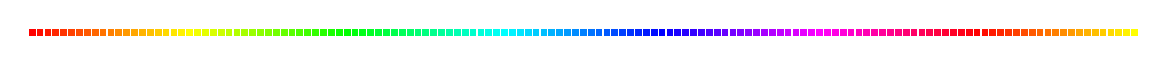
\begin{tikzpicture}[x=1mm,y=1mm]
  \colorlet{color min hsb}[hsb]{red}
  \colorlet{color max hsb}[hsb]{magenta}
  \foreach \pos in {0,...,140}{
    \colorlet{my color hsb}[rgb]{color max hsb!\pos!color min hsb}
    \fill[fill=my color hsb,draw=white] (\pos,1) rectangle +(1mm,1mm);
  }
\end{tikzpicture}}

%%%%%%%%%%%%%%%%%
%%%%%%%%%% TITLE INFO
%%%%%%%%%%%%%%%%%
\title{Notes for Abstract Algebra}
\author{Nicholas Tomlin}
\date{\today}

%%%%%%%%%%%%%%%%%
%%%%%%%%% HEADER INFO
%%%%%%%%%%%%%%%%%
\pagestyle{fancy}
\lhead{Nicholas Tomlin}
\chead{}
\rhead{MATH 1530: Abstract Algebra}
\lfoot{}
\cfoot{\thepage}
\rfoot{}

%%%%%%%%%%%%%%%%%
%%%%%%%%%%% TESTING
%%%%%%%%%%%%%%%%%
\newcounter{examplecounter}
\renewcommand{\theexamplecounter}{\arabic{examplecounter}}

\newenvironment{example}[1]{%
\vspace{-0.35cm}
\rule{\linewidth}{0.1mm}

\refstepcounter{examplecounter}%
\noindent\textbf{Example~\theexamplecounter}:}
{\\[0.01in]\rule{\linewidth}{0.1mm}}

%%%%%%%%%%%%%%%%%%%%%%%%%%%%%%%%%%
%%%%%%%%%%%%%%%%%%%%%%%%%%%%%%%%%%
%%%%%%%%%% BEGIN DOCUMENT %%%%%%%%%%%%%
%%%%%%%%%%%%%%%%%%%%%%%%%%%%%%%%%%
%%%%%%%%%%%%%%%%%%%%%%%%%%%%%%%%%%
\begin{document}
% \maketitle
\thispagestyle{empty}
\begin{center}
\textsc{\Large MATH 1530: Abstract Algebra}\\[0.4cm]
\textsc{\large Spring 2017}\\[0.2cm]

\HRuleRed\\[0.4cm]
{ \huge \bfseries Notes for Abstract Algebra}\\[0.1cm]
\HRuleRed\\[0.2cm]

\Large \textsc{Nicholas Tomlin}
\end{center}
\tableofcontents
\newpage

%%%%%%%%%%%%%%%%%
%%%%%% SECTION: GROUPS
%%%%%%%%%%%%%%%%%
\section{Introduction}
\subsection{Preliminary definitions}

\begin{definition}{}{}
A \textbf{set} is ``a collection of elements," e.g., the integers $\Z = \{\ldots,-2,-1,0,1,2,\ldots\}$, the real numbers $\R$, and the rational numbers $\Q$ (fractions). Note that we use $\Z_{\ge 0} = \{0,1,2,\ldots\}$ to refer to the nonnegative integers.
\end{definition}

\begin{definition}{}{}
If $A,B$ are sets, define the \textbf{Cartesian product} as $$A \times B = \{(a,b) \ | \ a \in A, b \in B\}$$ We can abbreviate $A^2 = A \times A$. Similarly, if $A_1,\ldots,A_n$ are sets, then $$A_1 \times \dots \times A_n = \{(a_1,\ldots,a_n) \ | \ a_1 \in A_1, \ldots, a_n \in A_n\}$$ Let $A^n = A \times \dots \times A$ ($n$ times).
\end{definition}

\begin{definition}{}{}
A \textbf{function} $f : A \rightarrow B$, or a \textbf{map}, is an association of an element $f(a) \in B$ to every element $a \in A$. We call $A$ the \textbf{domain} of $f$, and $B$ the \textbf{codomain} of $f$. Furthermore, the \textbf{range} or \textbf{image} of $f$ is $$\{f(a) : a \in A\}$$
\end{definition}
\begin{example}{}
Let $f : \Z \rightarrow \Z$ be given by $x \mapsto 2x$.\footnote{The symbol $\mapsto$ means "maps to."} The codomain and domain are both $\Z$, while the image is $$\{b \in \Z : b = 2a \text{ for some } a\in\Z \}$$ which is the set of even numbers.
\end{example}

\begin{definition}{}{}
A \textbf{binary operation} on a given set $G$ is a function $* : G \times G \rightarrow G$. For example, integer addition $(+ : \Z \times \Z \rightarrow \Z)$ is a binary operation.
\end{definition}

\subsection{What is a group?}

\begin{definition}{}{}
A \textbf{group} is a set $G$ together with a binary operation $* : G \times G \rightarrow G$ such that the following hold:
\begin{enumerate}[(1)]
\item ``Associativity": for $a,b,c \in G$, $(a*b)*c = a*(b*c)$.
\item ``Existence of the identity": there is an element $e \in G$ such that for all $g \in G$, $e*g = g$ and $g*e = g$.
\item ``Existence of inverses": for every $g \in G$, there is an element that we'll call $g^{-1} \in G$ such that $g*g^{-1}=g^{-1}*g=e$, where $e$ is an identity element of $G$.
\end{enumerate}
\end{definition}

\begin{theorem}{}{}
$(\Z,+)$ forms a group.\footnote{We write the ordered pair $(\Z,+)$ to represent the integers along with the binary operation of addition.}
\end{theorem}

\begin{proof}
Indeed, we check that $(\Z,+)$ satisfies the three axioms of being a group:
\begin{enumerate}[(1)]
\item For associativity, we note that $(a+b)+c = a+(b+c)$ for all $a,b,c \in \Z$.
\item For existence of the identity, $0 \in Z$ satisfies $0 + a = a+0 = a$ for all $a \in \Z$.
\item For existence of inverses, consider some $a \in \Z$. Then assert that $-a \in \Z$ satisfies $a+(-a)=(-a)+a=0$.
\end{enumerate}
Thus, we have shown that $(\Z,+)$ is a group.
\end{proof}

\begin{definition}{}{}
Let $(G,*)$ be a group. Then $G$ is a \textbf{commutative} or \textbf{abelian} group if $a*b = b*a$ for all $a,b \in G$.
\end{definition}

For example, $\Z$, $\R$, and $\Q$ with addition are all \textbf{commutative groups}. However, below is an example of a non-commutative group.

\begin{example}{}{}
Not all groups are commutative. Let $G$ be the symmetries of a can (cylinder) $C$ which are physically possible, i.e., the rigid motions preserving the can. These are called the orientation-preserving isometries of $\R^3$. More precisely, we can define the set of symmetries $$\text{Sym}(C) = \{A : \R \rightarrow \R : \text{ det}(A)=1, A(C)=C \}$$ where $A$ is an linear transformation which is an isometry. Put this together with the binary operation of composition $\circ$, and this forms a group.

However, these motions are not commutative. That is, flipping the can and then rotating it is distinct from rotating the can and then flipping it.
\end{example}

\begin{theorem}{}{}
Every group has a unique identity element.
\end{theorem}

% Section 1.3
\subsection{The group $\Z/n\Z$}
\begin{definition}{}{}
Let $A$ be a nonempty set. Then a \textbf{relation} on $A$ is a subset $R \subseteq A \times A$, which is written $a \sim b$ if and only if $(a,b) \in R$.
\end{definition}
\begin{definition}{}{}
A relation $R$ is an \textbf{equivalence relation} if it satisfies the following three properties:
\begin{enumerate}[(1)]
\item ``Reflexivity": $a \sim a$ for all $a \in A$.
\item ``Symmetry": if $a\sim b$, then $b\sim a$ for all $a,b \in A$.
\item ``Transitivity": if $a\sim b$ and $b\sim c$, then $a\sim c$ for all $a,b,c \in A$.
\end{enumerate}
\end{definition}
Let $f: A \rightarrow D$ be a function. Given $a,b \in A$, we'll say $a\sim b$ if and only if $f(a)=f(b)$. This is an equivalence relation; moreover, all equivalence relations can be written in this form.

\begin{example}{}{}
Consider the set $A = \{\text{students in Math 1530}\}$. For any two students $a,b \in A$, say $a\sim{b}$ if and only if $a$ has the same birthday as $b$. This is an equivalence relation, so we can relate this to the above form as follows. Let $D = \{\text{Jan 1,}\ldots\text{, Dec 31}\}$ be the set of possible birthdays, and $f : A \rightarrow D$ be a function mapping students to their birthdays.
\end{example}
\begin{definition}{}{}
Let $\sim$ be an equivalence relation on $A$. Then we say $$\overline{a} = \{b \in A : a \sim b\}$$ is an \textbf{equivalence class} of $a$. The equivalence classes of $A$ partition it into non-overlapping groups covering all of $A$.
\end{definition}

Let $n \in \Z$. Say $n \mid a$ (pronounced ``$n$ divides $a$") if $a = kn$ for some $k \in \Z.$ Now define a relation $\equiv_n$ on $\Z$ by $a\equiv_nb$ if $n\mid (a-b)$. We call this relation ``congruent modulo $n$." To prove that $\equiv_n$ is an equivalence relation on $\Z$, we must show the following:
\begin{enumerate}[(1)]
\item $a \equiv_na$ for all $a\in\Z$. \cm{Indeed, $a-a=0$ and $n\mid 0$.}
\item $a\equiv_nb$ implies $b\equiv_na$ for all $a,b\in\Z.$
\item $a\equiv_nb$ and $b\equiv_nc$ implies $a\equiv_nc$ for all $a,b,c\in\Z.$
\end{enumerate}
\begin{proof}
Indeed, we will show that $\equiv_n$ satisfies the three axioms of equivalence relations:
\begin{enumerate}[(1)]
\item For reflexivity, $a-a=0$ and $n\mid 0$.
\item For symmetry, $a\equiv_n b \implies n\mid (a-b) \implies a-b=kn$ for some $k\in\Z$. We want to show that $b\equiv_n a$, i.e., $b-a=ln$ for some $l\in\Z$. We may take $l=(-k)$.
\item For transitivity, there exists $k,l\in\Z$ such that $a-b=kn$ and $b-c=ln$. Then, adding these equations gives $a-c=(k+l)n$. Since $(k+l)\in\Z$, we conclude $n\mid (a-c) \implies a\equiv_nc$.
\end{enumerate}
\end{proof}

\begin{definition}{}{}
$\Z/n\Z$ is the set of equivalence classes modulo $n$, i.e., equivalence classes with respect to the equivalence relation $\equiv_n$.
\end{definition}

For example, $\Z/5\Z = \{\overline{0}, \overline{1}, \overline{2}, \overline{3}, \overline{4}\}$. The choice of ``captains" is not important, so we could alternatively write this as $\Z/5\Z = \{ \ol{10}, -\ol{4}, \ol{2}, \ol{8}, \ol{24} \}$.
\begin{definition}{}{}
We define the binary operation of addition $+: \Z/n\Z \times \Z/n\Z \rightarrow \Z/n\Z$ as follows: $\overline{a}+\overline{b} = \overline{a+b}$ for all $\overline{a}, \overline{b} \in \Z/n\Z$.
\end{definition}
\begin{lemma}{}{}
Addition on $\Z/n\Z$ is well-defined, as stated above.
\end{lemma}
\begin{proof}
Given $a_1,a_2 \in \Z$ such that $\overline{a}_1 = \overline{a}_2$ and $b_1,b_2 \in \Z$ such that $\overline{b}_1 = \overline{b}_2$, we want to show that $\overline{a_1+b_1} = \overline{a_2+b_2}$. Indeed, $a_1-a_2 = kn$ and $b_1-b_2 = ln$ for $k,l\in\Z$. Adding these equations gives $$(a_1+b_1) - (a_2+b_2) = (k+l)n$$ so that $\overline{a_1+b_1} = \overline{a_2+b_2}$ since $(k+l)\in\Z$.
\end{proof}
\begin{theorem}{}{}
$(\Z/n\Z, +)$ is a group.
\end{theorem}
\begin{proof}
Again, we check the three group axioms:
\begin{enumerate}[(1)]
\item We have 
\begin{align*}
\overline{a}+(\overline{b}+\overline{c}) &= \overline{a} + \overline{b+c} \\
&= \overline{a + (b+c)} \\
&= \overline{(a+b) +c} \\
&= \overline{a+b} + \overline{c} \\
&= (\overline{a} + \overline{b}) + \overline{c}
\end{align*}
by associativity of addition.
\item We have $\overline{0} + \overline{a} = \overline{a} + \overline{0} = \overline{a}$ for all $a \in \Z/n\Z$.
\item We have $-\overline{a} + \overline{a} = \overline{a} + (-\overline{a}) = \overline{0}$ for all $a \in \Z/n\Z$.
\end{enumerate}
\end{proof}
\begin{definition}{}{}
We define the binary operation of multiplication $\cdot: \Z/n\Z \times \Z/n\Z \rightarrow \Z/n\Z$ as follows: $\overline{a}\cdot \overline{b} = \overline{ab}$ for all $\overline{a}, \overline{b} \in \Z/n\Z$.
\end{definition}
\begin{theorem}{}{}
Multiplication on $\Z/n\Z$ is well-defined, as defined above.
\end{theorem}

\subsubsection{The multiplicative group $(\Z/n\Z)^{\times}$}
However, $(\Z/n\Z, \cdot)$ is not a group unless $n=1$, as inverses may not exist. Indeed, $\bar{1}$ is an identity, but $\bar{0}\cdot a = \bar{1}$ has no solution, i.e.,  there is no multiplicative inverse for $\bar{0}$. Now, let: $$(\Z/n\Z)^{\times} = \{ \bar{a} \in \Z/n\Z : \bar{a}\cdot\bar{c} = \bar{1} \text{ for some } \bar{c}\in\Z/n\Z \}$$
We call this set ``the multiplicative units of $\Z/n\Z$."

\begin{example}{}{}
Given $n=4$, we say $(\Z/4\Z)^{\times} = \{ \bar{1}, \bar{3} \}$. In particular, $\bar{1} \cdot \bar{1} = \bar{1}$ and $\bar{3} \cdot \bar{3} = \bar{1}$.
\end{example}
\begin{theorem}{}{}
$((\Z/n\Z)^{\times}, \cdot)$ is a group.
\end{theorem}
\begin{proof}
Given $\bar{a}, \bar{c} \in (\Z/n\Z)^{\times}$, we must show that $\bar{a} \cdot \bar{c} \in (\Z/n\Z)^{\times}$. First, we will show that $\cdot$ defines a binary operation on $(\Z/n\Z)^{\times}$, i.e., ($\Z/n\Z)^{\times}$ is closed under multiplication. Indeed, $\bar{a} \cdot \bar{b} = \bar{1}$ and $\bar{c} \cdot \bar{d} = \bar{1}$ for some $\bar{b}, \bar{d} \in \Z/n\Z$. Multiplying these equations gives:
\begin{align*}
\bar{1} &= (\bar{a}\cdot\bar{b})(\bar{c}\cdot\bar{d}) \\
&= (\bar{a}\cdot\bar{c})(\bar{b}\cdot\bar{d})
\end{align*}
In addition, associativity holds as in $\Z/n\Z$. There is an identity element, namely $\bar{1}$, and inverses exist as in $\Z/n\Z$ based on the definition of $(\Z/n\Z)^{\times}$.
\end{proof}
\begin{theorem}{}{}
$(\Z/n\Z)^{\times} = \{ \bar{a} : a \in \Z, (a,n) = 1 \}$
\end{theorem}
\subsubsection{Applications of arithmetic in $\Z/n\Z$}
\begin{example}{}{}
\textit{What is the last digit of $2^{50}$?} To calculate this, work in $\Z/10\Z$:
\begin{align*}
\bar{2} \cdot \bar{2} &= \bar{4} \\
\bar{2} \cdot \bar{2} \cdot \bar{2} &= \bar{8} \\
\bar{2} \cdot \bar{2} \cdot \bar{2} \cdot \bar{2} &= \bar{6} \\
\bar{2} \cdot \bar{2} \cdot \bar{2} \cdot \bar{2} \cdot \bar{2} &= \bar{2}
\end{align*}
and so on. Hence this cycles through ($\bar{2}, \bar{4}, \bar{8}, \bar{6}$) as demonstrated above. We can use this pattern to see the last digit is \boxed{4}. Alternatively, since $\overline{2^5} = \bar{2}$:
\begin{align*}
\overline{2^{50}} &= \overline{(2^5)^{10}} \\
&= \overline{2^{10}} \\
&= \overline{2^5} \cdot \overline{2^5} \\
&= \bar{2} \cdot \bar{2} = \bar{4}
\end{align*}
\vspace{-0.8cm}
\end{example}
% 1.4
\subsection{Some general theorems about groups}
\begin{lemma}{}{}
Let $(G, *)$ be a group. Then $G$ has a unique identity element.
\end{lemma}
\begin{proof}
Let $e,f \in G$ be identity elements. Then:
\begin{align*}
e = e*f &\text{ (since $f$ is an identity element)} \\
e*f = f &\text{ (since $e$ is an identity element)}
\end{align*}
Therefore $e=f$ and there is exactly one identity element.
\end{proof}
\begin{lemma}{}{}
Let $(G, *)$ be a group. Then $G$ has a unique inverse.
\end{lemma}
\begin{proof}
Given $a \in G$, suppose that $b,c \in G$ are inverses of $a$. Then:
\begin{align*}
e &= a*b \text{ (since $b$ inverse of $a$)} \\
c*e &= c*a*b \\
c &= b \text{ (since $c$ inverse of $a$)}
\end{align*}
Since $b=c$, every element of a group must have a unique inverse.
\end{proof}
\begin{lemma}{}{}
Let $(G, *)$ be a group. Then $(a*b)^{-1} = (b^{-1})*(a^{-1})$ for all $a,b \in G$.
\end{lemma}
\begin{proof}
We need to check that $(a*b)*((b^{-1})*(a^{-1})) = e$ is the identity element. This is left as an exercise to the reader.
\end{proof}
\begin{lemma}{}{}
Let $(G, *)$ be a group. For any $a_1,\ldots,a_n \in G$, $a_1*\dots *a_n$ has a well-defined value, i.e., is independent of bracketing.
\end{lemma}
\begin{theorem}{}{}
Given $(G, *)$ a group and $a,b \in G$, the equation $ax=b$ has a unique solution.
\end{theorem}
\subsection{The order of a group}
\begin{definition}{}{}
Let $(G,*)$ be a group. The \textbf{order of a group} $G$ denoted $|G|$ is the number of elements. If $G$ is infinite, say $|G| = \infty$.
\end{definition}
\begin{definition}{}{}
Let $(G,*)$ be a group. The \textbf{order of an element} $a \in G$ is the smallest $n \in \Z_{> 0}$ such that $a^n = e$. 
\end{definition}
\begin{example}{}{}
The symmetries of a can $Sym(C)$ has order $|Sym(C)| = \infty$, but it has elements of finite order. For instance, the identity has order $|e| = 1$. A rotation by $180^{\circ}$ has order $2$, a rotation by $120^{\circ}$ has order $3$, and so on. In fact, for any order $n \in \Q$, a rotation by $2\pi/n$ has order $n$.
\end{example}

\subsection{A brief interlude on functions}
\begin{definition}{}{}
Let $f : A \rightarrow C$ be a function on sets. Then $f$ is \textbf{injective} (one-to-one) if given any two elements $a,b \in A$, then $f(a)=f(b) \implies a=b$.\footnote{The contrapositive, $a \ne b \implies f(a) \ne f(b)$ is equivalent.}
\end{definition}
\begin{definition}{}{}
Let $f : A \rightarrow C$ be a function on sets. Then $f$ is \textbf{surjective} (onto) if for all $c\in C$, there exists $a\in A$ with $f(a)=c$.
\end{definition}
\begin{definition}{}{}
A function is \textbf{bijective} if it is both injective and surjective.
\end{definition}
Given a function $f : A \rightarrow C$ between finite sets $A$ and $C$, then we write $|A|$ to denote the number of elements (i.e., the \textbf{cardinality}) of $A$. Then, we can say:
\begin{enumerate}
\item $f$ injective $\implies |A| \le |C|$
\item $f$ surjective $\implies |A| \ge |C|$
\item $f$ bijective $\implies |A| = |C|$
\end{enumerate}

\section{Some important groups}
\subsection{Dihedral groups}
\begin{definition}{}{}
The \textbf{dihedral group}, denoted $D_{2n}$, is the group of rigid motions of a regular $n$-gon. The group operation is composition.
\end{definition}
The $2n$ subscript in the name for the dihedral group refers to the order of the group. We can rotate the $n$-gon by integer multiples of $2\pi/n$, and we can ``flip" the $n$-gon in $\R^3$. These combinations of rotations and flips are specifically the $2n$ elements of the dihedral group.

More rigorously, we can label the vertices of an $n$-gon $\{1,\ldots,n\}$ in clockwise order. A rigid motion of the $n$-gon can be recorded as a bijection $$\sigma : \{1,\ldots,n\}\rightarrow\{1,\ldots,n\}$$
i.e., a permutation of $\{1,\ldots,n\}$. Therefore, $\sigma(j)$ records the new position of vertex $j$. We claim that the map of sets $$D_{2n}\rightarrow \{\text{bijections from } \{1,\ldots,n\} \rightarrow \{1,\ldots,n\}\}$$
is injective. The intuition here is that the rigid motions of the $n$-gon are a subset of the possible permutations. Now, note that $D_{2n}$ has at least $2n$ elements (as shown above).
\begin{theorem}{}{}
$|D_{2n}| = 2n$ (i.e., $D_{2n}$ is the dihedral group of order $2n$)
\end{theorem}
\begin{proof}
We know that $|D_{2n}| \ge 2n$, so we want to show $|D_{2n}| \le 2n$. Define a map:
\begin{align*}
D_{2n} &\rightarrow \{ (1,2),\ldots,(n-1,n), (n,1), (2,1), \ldots, (n,n-1), (1,n) \} \\
\sigma &\mapsto (\sigma(1), \sigma(2))
\end{align*}
where the target has cardinality $2n$. This map is injective, since any two adjacent elements uniquely define a rigid motion of the $n$-gon. Thus, $|D_{2n}| \le 2n$.
\end{proof}

\subsubsection{Explicit description of $D_{2n}$}

Label an $n$-gon $\{1,\ldots,n\}$ on its vertices. Let $r$ be clockwise rotation by $2\pi/n$, and let $s$ be a reflection about the central line bisecting the angle at vertex $1$. Note that:
\begin{itemize}
\item $1, \ldots, r^{n-1} \in D_{2n}$ are distinct rotations.
\item $s$ is distinct from $1, \ldots, r^{n-1}$.
\item $s,sr,sr^2,\ldots,sr^{n-1} \in D_{2n}$ are all distinct.
\end{itemize}
\begin{theorem}{}{}
$D_{2n} = \{1,\ldots,r^{n-1}, s, \ldots, sr^{n-1}\}$
\end{theorem}
\begin{proof}
We need only show that $$r^i \ne sr^j \text{ for any } i,j \in \{1,\ldots,n-1\}$$ Indeed, $r^{i-j} \ne s$.
\end{proof}
Furthermore, $rs = sr^{-1}$, i.e., rotating and reflecting is the same as reflecting and rotating by the same amount in the opposite direction.

\newpage
Given these observations, we now know how to multiply in $D_{2n}$. For example, we can multiply the rigid motions $(sr^6)$ and $(sr^9)$ on an arbitrary regular $n$-gon:
\begin{align*}
(sr^6)(sr^9) &= s(r^6s)r^9 \\
&= s(r^5sr^{-1})r^9 \\
&= s(sr^{-6})r^9 \\
&= r^3
\end{align*}
Alternatively, we can define $D_{2n}$ in terms of generators and relations as follows:
$$D_{2n} = \langle r,s \ | \ r^n = 1, s^2 = 1, rs=sr^{-1} \rangle$$
In particular, any relation on elements of $D_{2n}$ can be obtained from the given relations.

\subsection{Symmetric groups}
\begin{definition}{}{}
Let $X$ be a non-empty set, and let $S_X$ be the permutations of $X$. When $X = [n] := \{1,\ldots,n\}$, we write $S_n = S_{\{1,\ldots,n\}}$. Then $S_X$ is a group under composition, where $f*g = g\circ f$.
\end{definition}
\begin{example}{}{}
$S_3 = \{\{1,2,3\}, \{1,3,2\}, \{2,1,3\}, \{2,3,1\}, \{3,1,2\}, \{3,2,1\}\}$.
\end{example}
\begin{lemma}{}{}
A map $f : A \rightarrow C$ is a bijection if and only if there exists a function $g : C \rightarrow A$ such that $f\circ g = \operatorname{id}_C$ and $g\circ f = \operatorname{id}_C$.
\end{lemma}

\begin{theorem}{}{}
The order $|S_n| = n!$, i.e., the factorial of $n$.
\end{theorem}
\begin{proof}
To choose a permutation of $\{1,\ldots,n\}$, we can choose any of $n$ mappings for $1$, $n-1$ remaining mappings for $2$, and so on. Since there is no ``overlap,'' this is an injective function. Furthermore, since this is injective and the domain and range have the same number of elements, it is also a bijection.
\end{proof}
\newpage
\subsubsection{Cycle notation for permutations}
Let $\sigma \in S_n$. Using the two-line notation style for permutations, we can write:
$$\sigma = \begin{pmatrix}
1 & 2 & 3 & 4 & 5 & 6 & 7 \\
7 & 2 & 4 & 1 & 6 & 5 & 3
\end{pmatrix}$$
This maps $1\mapsto 7$, $2\mapsto 2$, and so on. Alternatively, it can be represented with a directed graph, as in the following example:

\begin{example}{}{}
Given $\sigma = \{7 , 2 , 4 , 1 , 6 , 5 , 3\}$, the corresponding directed graph is as follows:
\begin{center}
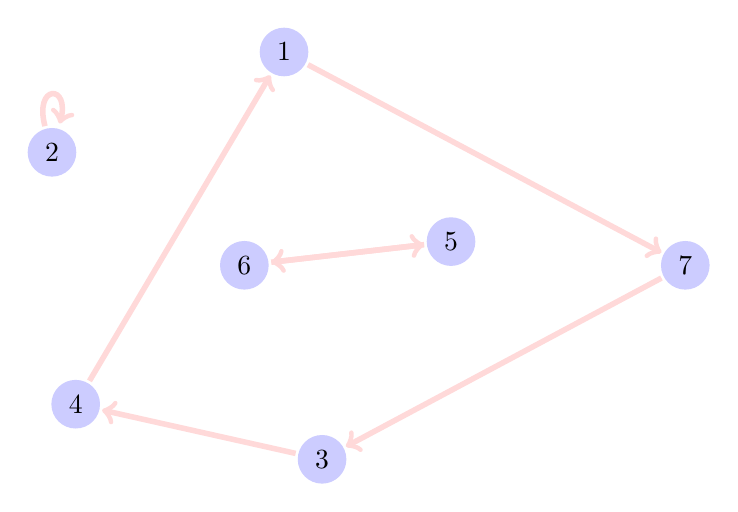
\begin{tikzpicture}[line width=2pt, scale=0.7] 
	\tikzstyle{every node} = [circle, fill=blue!20]
	\node (1) at (0.72, 3.87) {1};
	\node (4) at (-3.06, -2.52) {4};
	\node (3) at (1.41, -3.52) {3};
	\node (2) at (-3.49, 2.05) {2};
	\node (5) at (3.75, 0.43) {5};
	\node (6) at (0,0) {6};
	\node (7) at (8,0) {7};
	\draw [->, pink!60] (1)--(7);
	\draw [->, pink!60] (7)--(3);
	\draw [->, pink!60] (3)--(4);
	\draw [->, pink!60] (4)--(1);
	\draw [->, pink!60] (5)--(6);
	\draw [->, pink!60] (6)--(5);
	\path (2) edge [pink!60, loop above] (2);
\end{tikzpicture}
\end{center}
The above directed graph can be divided into three disjoint cycles $\sigma = (1734)(56)(2)$, or just $\sigma = (1734)(56)$.\footnote{It is a convention to remove $1$-element cycles from the notation, just as a convenience. The order of these cycles is not important, and $\sigma$ could equivalently be written as $\sigma = (65)(3417)$, or one of many other possible combinations.} More generally, we'll claim that any such permutation must produce a graph of disjoint cycles. This notation allows us to calculate inverses and powers:
\begin{itemize}
\item \textbf{Inverses} - $\sigma^{-1} = (4371)(65)$, which is calculated by going in the reverse direction
\item \textbf{Powers} - $\sigma^{2} = (13)(47)(5)(6) = (13)(47)$, where we count every other element of each cycle. To calculate $\sigma^{n}$, count every $n$th element.
\end{itemize}
\fakeline
\end{example}
\begin{theorem}{}{}
Let $\sigma \in S_n$. Then, draw an arrow from $i$ to $\sigma(i)$ for each $i \in \{1,\ldots,n\}$. The resulting directed graph is a collection of disjoint cycles.
\end{theorem}
\begin{theorem}{}{}
In general, for $\sigma \in S_n$, $|\sigma|$ is the least common multiple of all cycle lengths in the cycle decomposition of $\sigma$.
\end{theorem}
\begin{definition}{}{}
Say that $\sigma \in S_n$ is an \textbf{m-cycle} if its cycle notation has just one cycle of length $m$ (and all other cycles length $1$).
\end{definition}
We can also use this notation to calculate products (i.e., composition) of permutations. For example, consider the case of $(154)(23) \circ (12345)$:\footnote{$\sigma \circ \tau$ means first $\tau$, then $\sigma$} since $1 \mapsto 2$ in $(12345)$ and then $2\mapsto 3$ in $(154)(23)$, it must be the case that $1\mapsto 3$ in their composition. This general principle can be applied repeatedly to calculate that
\begin{align*}
(154)(23) \circ (12345) &= (13)(2)(4)(5) = (13) \\
(1734) \circ (56) &= (1734)(56)
\end{align*}
where in the second example, composition is nothing more than concatenation since the two permutations are non-overlapping. Such disjoint cycles always commute, but not all permutations commute. For example, $(12) \circ (13) = (132)$ but $(13) \circ (12) = (123)$.
\begin{theorem}{}{}
$S_n$ is nonabelian for $n \ge 3$.
\end{theorem}
\subsection{Homomorphisms and isomorphisms}
\subsubsection{Motivation}
Consider the following groups:
\begin{enumerate}[1.]
\item $(\Z/2\Z,+) = \{\bar{0}, \bar{1}\}$
\begin{multicols}{2}
\begin{itemize}
\item $\bar{0}+\bar{0}=\bar{0}$
\item $\bar{0}+\bar{1}=\bar{1}$
\end{itemize}
\begin{itemize}
\item $\bar{1}+\bar{0}=\bar{1}$
\item $\bar{1}+\bar{1}=\bar{0}$
\end{itemize}
\end{multicols}
\item $S_2 = \{ \text{id}, (12) \}$, with $\circ$:
\begin{multicols}{2}
\begin{itemize}
\item $\text{id}\circ\text{id}$ = id
\item $\text{id}\circ(12) = (12)$
\end{itemize}
\begin{itemize}
\item $12\circ\text{id}=(12)$
\item $(12)\circ(12)=\text{id}$
\end{itemize}
\end{multicols}
\item A group $(P,+)$ with elements $P = \{\text{even, odd}\}$, with $+$ given by:
\begin{multicols}{2}
\begin{itemize}
\item even + even = even
\item even + odd = odd
\end{itemize}
\begin{itemize}
\item odd + even = odd
\item odd + odd = even
\end{itemize}
\end{multicols}
\end{enumerate}
Are these groups all the same? Not exactly (they have different elements), but they are all \textit{isomorphic}. This is described formally in the next section.
\subsubsection{Formal definitions and theorems}
\begin{definition}{}{}
A \textbf{homomorphism} of groups $(G,*)$ and $(H,\cdot)$ is a map $\phi : G \rightarrow H$ such that for all $g,g' \in G$, $\phi(g) \cdot \phi(g') = \phi(g*g')$. Equivalently, for all $a,b,c \in G$, if $a*b = c$, then also $\phi(a)\cdot\phi(b)=\phi(c)$.
\end{definition}

\begin{example}{}{}
Given groups $G$ and $H$, there is always a homomorphism
\begin{align*}
\phi : \ &G \rightarrow H \\
&g \mapsto e \text{ (identity in $h$)}
\end{align*}
Then $\phi$ is a homomorphism since $\phi(g_1)\cdot \phi(g_2) = \phi(g_1g_2) = \phi(e)$.
\end{example}

\begin{definition}{}{}
Let $(G,*)$ and $(H,\cdot)$ be groups. An \textbf{isomorphism} is a map $\phi : G \rightarrow H$ such that the following are true:
\begin{itemize}
\item $\phi$ is a bijection.
\item for all $g,g' \in G$, $\phi(g) \cdot \phi(g') = \phi(g*g')$.
\end{itemize}
In this case, we say that $G \cong H$. An isomorphism is a bijective homomorphism.
\end{definition}
\begin{example}{}{}
Here are some examples of isomorphisms:
\begin{itemize}
\item $G \cong G$ via identity map.
\item Consider the exponential function $\operatorname{exp} : \R \rightarrow \R_{>0}$ bijection taking addition to multiplication: $e^{x+y}=e^xe^y$. This yields the isomorphism $(\R,+) \cong (\R_{>0}, \cdot)$.
\end{itemize}
\fakeline
\end{example}
\begin{theorem}{}{}
If $G\cong H$ and $G$ is abelian, then $H$ is abelian.
\end{theorem}
\begin{lemma}{}{}
Let $\phi : G \rightarrow H$ be a homomorphism. Then $\phi(e_G) = e_H$.
\end{lemma}
\begin{proof}
Indeed, $\phi(e_G) = \phi(e_Ge_G) = \phi(e_G)\phi(e_G)$. Given $x\in H$ a group, $x\cdot x = x$ if and only if $x$ is the identity. Thus $\phi(e_G) = e_H$.
\end{proof}
\begin{lemma}{}{}
Let $\phi : G \rightarrow H$ be a homomorphism. Then for all $a\in G$, $\phi(a^{-1}) = \phi(a)^{-1}$.
\end{lemma}
\begin{proof}
Given $a\in G$, $\phi(e_G) = \phi(a \cdot a^{-1}) = \phi(a)\phi(a^{-1}) = e_H$ by the previous lemma. Therefore, $\phi(a^{-1}) = \phi(a)^{-1}$.
\end{proof}
\subsubsection{Homomorphisms of $\Z$}
Let $H$ be any group. What are the homomorphisms $\Z \rightarrow H$? We claim that given $b \in H$, there is a unique homomorphism $\phi : \Z \rightarrow H$ with $\phi(1) = b$. This means that a homomorphism $\Z \rightarrow H$ exists and is uniquely determined by the element it sends $1$ to.
\begin{theorem}{}{}
Let $H$ be any group. Then given an element $b \in H$, there exists a unique homomorphism $\phi$ from the additive group $(\Z,+)$ to $H$ such that $\phi(1) = b$.
\end{theorem}
\begin{proof}
For uniqueness, if $\phi : \Z \rightarrow H$ with $\phi(1) = b$, then $\phi(1 + 1) = \phi(1)\phi(1) = b^2$. Continuing in this way, $\phi(1 + \cdots + 1) = \phi(1) \cdots \phi(1) = b^n$. Furthermore, $\phi(0) = e_H$ and $\phi(-1) = b^{-1}$; as before, $\phi(-n) = b^{-n}$. Thus $\phi(n) = b^n$ for all $n \in \Z$. For existence, we'll show that the following is a homomorphism:
\begin{align*}
\phi : \ &\Z \rightarrow H \\
&n \mapsto b^n
\end{align*}
Indeed, given $x,y \in \Z$, then $\phi(x)\phi(y) = b^xb^y = b^{x+y} = \phi(x+y)$ as desired.
\end{proof}

\subsection{Subgroups}
\begin{definition}{}{}
Let $G$ be a group. A subset $H \subseteq G$ is a \textbf{subgroup} of $G$ if:
\begin{itemize}
\item $H \ne \emptyset$
\item Given $g_1,g_2 \in H$, then $g_1g_2 \in H$.
\item Given $g \in H$, $g^{-1} \in H$.
\end{itemize}
Equivalently, the operator on $G$ restricts to an operation on $H$, and $H$ is a group with respect to this. Write $H \le G$ if this is true.
\end{definition}
\begin{example}{}{}
Here are some examples of subgroups (and non-subgroups):
\begin{enumerate}
\item The additive group $2\Z = \{\ldots,-2,0,2,\ldots\}$ is a subgroup of $\Z$; this holds for any $n\Z$.
\item $\Z_{\ge 0} = \{0,1,2,\ldots\} \subseteq \Z$ is not a subgroup since additive inverses do not exist.
\item For any group $G$, $G$ and the trivial subgroup $e_G$ are always groups.
\end{enumerate}
\fakeline
\end{example}
\begin{lemma}{Subgroup Criterion}{}
Given a group $G$, say $H \subseteq G$ for some nonempty subset $H$. Then $H$ is a subgroup if for all $x,y \in H$, $xy^{-1} \in H$.
\end{lemma}
\begin{definition}{}{}
Let $G$ be a group. We define the \textbf{center} of $G$ as
$$Z(G) = \{g\in G : gx = xg \text{ for all } x\in G\}$$
If $G$ is abelian, then $Z(G)=G$ and conversely $Z(G)=G \implies G$ is abelian.
\end{definition}
\begin{theorem}{}{}
The center of a group is always a subgroup, i.e., $Z(G) \le G$ for any $G$.
\end{theorem}
\begin{proof}
Given $x,y \in Z(G)$, we want to show that $xy^{-1} \in Z(G)$. Namely, given $z \in G$, we want $(xy^{-1})z = z(xy^{-1})$. Indeed, since $x,y$ commute with all members of $G$:
\begin{align*}
(xy^{-1})z &= x(y^{-1}z) \\
&= (y^{-1}z)x \\
&= (z^{-1}y)^{-1}x \\
&= (yz^{-1})^{-1}x \\ 
&= (zy^{-1})x \\
&= z(y^{-1}x) \\
&= z(xy^{-1})
\end{align*}
as desired. Hence, the center of a group is always a subgroup.
\end{proof}
\subsection{Generators}
\begin{definition}{}{}
Let $G$ be a group, and let $S \subseteq G$ be any subset. Then the subgroup \textbf{generated by} $S$, denoted $\langle S \rangle$, is the collection of all (finite) products\footnote{We say $e$ is the product of exactly $0$ elements.} of elements in $S$ and their inverses in $G$.
If $\langle S \rangle = G$, we say $S$ \textbf{generates} $G$.
\end{definition}
\begin{example}{}{}
In $\Z$, $\langle 1 \rangle = \Z$. Furthermore, $\langle 3,4 \rangle = \Z$ since $4-3 = 1$, which has already been shown to generate $\Z$. However, $\langle 2 \rangle = 2\Z$ does not generate $\Z$. Notice that $\langle a,b \rangle = \Z$ if and only if $a,b$ are relatively prime.
\end{example}
\begin{theorem}{}{}
The generated set $\langle S \rangle$ is a subgroup.
\end{theorem}
\begin{theorem}{}{}
The subgroup $\langle S \rangle$ is the smallest subgroup of $G$ containing $S$.\footnote{That is, for any subgroup $H\le G$ such that $S \subseteq H$, then $\langle S \rangle \subseteq H$.}
\end{theorem}
\begin{proof}
Indeed, given a subgroup $H\le G$ with $S \subseteq H$, then $H$ must contain all products of elements in $S$ as well as inverses. Hence, $\langle S \rangle \subseteq H$.
\end{proof}

% 
\subsubsection{Properties of $\Z$}
Recall that $\Z = \{\ldots,-2,-1,0,1,2,\ldots\}$ is generated by a single element $\langle 1 \rangle$:
\begin{itemize}
\item \textbf{Well-ordering principle} - Every nonempty subset of $\Z_{> 0}$ has a least element. 
\item For $a,b \in \Z$, say $a\mid b$ (``$a$ divides $b$") if $b=ac$ for some $c \in \Z$.
\item Given $a,b \in \Z - \{0\}$, there exists a unique integer $d \ge 1$ (called the \textbf{greatest common divisor}) such that:
	\begin{itemize}
	\item $d\mid a$ and $d\mid b$
	\item if $e\in\Z$ such that $e\mid a$ and $e\mid b$, then $e\mid d$
	\end{itemize}
We notate this as $d=\operatorname{gcd}(a,b) = (a,b)$.
\item Given $a,b \in \Z - \{ 0 \}$, there exists a unique integer $l \ge 1$ (called the \textbf{least common multiple}) such that:
	\begin{itemize}
	\item $a\mid l$ and $b\mid l$
	\item if $m\in\Z$ such that $a\mid m$ and $b\mid m$, then $l\mid m$
	\end{itemize}
We notate this as $l=\operatorname{lcm}(a,b) = [a,b]$.
\begin{theorem}{}{}
Given $a,b \in \Z$, the product $a\cdot b = (a,b)\cdot [a,b]$.
\end{theorem}
\item \textbf{Division algorithm} - Given $a,b\in\Z-\{0\}$, there exists unique $q,r\in\Z$ such that $a=bq+r$ and $0 \le r < b$.
\item \textbf{Euclidean algorithm} - repeated use of the division algorithm can be used to compute the greatest common denominator. For example:
\begin{align*}
39 &= 2(15) + 9 \\
15 &= 1(9) + 6 \\
9 &= 1(6) + 3 \\
6 &= 2(3) + 0
\end{align*}
so we conclude that the greatest common denominator $(39,15) = 3$.
\begin{theorem}{}{}
Given $a,b \in \Z - \{0\}$, compute the following steps:
\begin{align*}
a &= q_0b + r_0	&0& \le r_0 < b \\
b &= q_1r_0 + r_1	&0& \le r_1 \le r_0 \\
r_0 &= q_2r_1 + r_2	&0& \le r_2 \le r_1 \\
&\phantom{test}\vdots &&\phantom{test}\vdots \\
r_{k-2} &= q_kr_{k-1} + r_{k}	&0& \le r_{k} \le r_{k-1} \\
r_{k-1} &= q_{k+1}r_k + 0
\end{align*}
We make the following three claims about this algorithm:
\begin{enumerate}
\item The algorithm terminates.
\item $r_k = ma + nb$ for some $m,n \in \Z$
\item $r_k = (a,b)$
\end{enumerate}
\end{theorem}
\begin{proof}
Indeed, we'll show the three claims:
\begin{enumerate}
\item Suppose for the sake of contradiction that the algorithm doesn't terminate. Then the sequence $r_0 > r_1 > r_2 > \dots > 0$ has no least element, violating the well-ordering principle.
\item Working backwards along the Euclidean algorithm:
\begin{align*}
r_k 	&= r_{k-2} - q_kr_{k-1} \\
	&= r_{k-2} - q_k(r_{k-3}-q_{k-1}r_{k-2}) \\
	&\phantom{testing}\vdots \\
	&= am + bn
\end{align*}
where we reach the final form by iterating substitution until the beginning of the algorithm.\footnote{As an aside, we can use this to write $3$ as a linear combination of $39$ and $15$:
\begin{align*}
3 &= 9 - 1(6) \\
&= 9 - 1(15-9) \\
&= 2(9) - 1(15) \\
&= 2(39-2\cdot 15) - 1(15)
\end{align*}
This gives us $3 = 2\cdot 39-5\cdot 15$ as desired.}
\item Note $r_k\mid r_{k-1}$ by the last equation. Also, $r_k\mid r_{k-2}$ by the second-to-last equation. Iterating this process, we get $r\mid a$ and $r\mid b$.

It remains to show that if $s \in \Z$, $s\mid a$, and $s\mid b$, then $s\mid r$. Indeed, $s\mid a$ and $s\mid b \implies s\mid(am+bn)$ for $m,n\in\Z$, so $s\mid r$ by (2).
\end{enumerate}
\end{proof}
\end{itemize}
\subsubsection{Cyclic groups}
\begin{definition}{}{}
A group $G$ is \textbf{cyclic} if it can be generated by a single element, i.e., $G = \langle x \rangle$ for some $x \in G$. Then $G = \{ x^n : n \in \Z \}$.
\end{definition}
\begin{example}{}{}
Here are some examples of cyclic groups (and non-cyclic groups):
\begin{itemize}
\item $\Z = \langle 1 \rangle = \langle -1 \rangle$ is a cyclic group.
\item $\Z/n\Z = \langle \bar{1} \rangle$ is also a cyclic group.
\item $\R/\Z$ is not a cyclic group. However, a dense cover can be generated by an irrational number. That is, for example, any element in $\R/\Z$ is arbitrarily close to but not confined in $\langle \pi \rangle$.
\item $D_{2n}$ is not cyclic.
\item Fix $n \ge 1$. Then $\{ z \in \C : z^n = 1 \}$ under multiplication is a cyclic group.
\item There are no uncountable cyclic groups.
\end{itemize}
\fakeline
\end{example}
\begin{lemma}{}{}
If $H = \langle x \rangle$, then $|H| = |x|$ (i.e., if $|x| = \infty$, then $|H| = \infty$)
\end{lemma}
\begin{proof}
First, consider the case that $|x| = n$ is finite. Then we claim that $$H = \{ 1,x,\ldots,x^{n-1} \}$$ and these are all distinct. If instead $x^a = x^b$ for some $x \le a < b < n$, then $1=x^{b-a}$, contradicting $|x| = n$. To show that $H$ does indeed equal this set,\footnote{In general, to show that any two sets $A$ and $E$ are equal, it is standard to show that $A \subseteq E$ and $E \subseteq A$.} we need to show that $H \supseteq \{ 1,x,\ldots,x^{n-1} \}$ (the reverse direction is by definition). Indeed, given $x^t \in H$ for some $t \in \Z$, then by the division algorithm $t = qn + r$ for some $0 \le r < n$. Then:
$$x^t = x^{qn+r} = x^{nq} x^r \in \{ 1,\ldots,x^n \}$$
Now, suppose $|x|$ infinite. Then, we'll claim $\{ \ldots, x^{-1},1,x,x^2,\ldots \}$ are all distinct. Indeed, if $x^a = x^b$ for $a < b$, then $x^{b-a} = 1$ is a contradiction.
\end{proof}
\begin{lemma}{}{}
Let $G$ be any group, and $x \in G$. If $x^m = 1$ and $x^n = 1$, then $x^{(m,n)} = 1$.
\end{lemma}
\begin{proof}
Let $d = (m,n)$. Note that $d = am + bn$ for $a,b \in \Z$. Then $x^d = x^{am}x^{bn} = 1$.
\end{proof}
\begin{lemma}{}{}
If $x^m = 1$, then $(|x|)\mid m$.
\end{lemma}
\begin{proof}
Let $n = |x|$. We want to show that $n\mid m$. If $m=0$, then indeed $n\mid m$. Otherwise, let $d = (m,n)$. Then by the previous lemma, $x^d = 1$ so $d \ge n$; hence $d = n$.
\end{proof}
\begin{theorem}{}{}
Let $G = \langle x \rangle = \{x^k : k \in \Z \}$. Then the following are true:
\begin{enumerate}
\item Let $|G| = n$. Then the map
\begin{align*}
\varphi : &\ G \to \Z/n\Z \\
&x^k \mapsto \bar{k}
\end{align*}
is well-defined and an isomorphism.
\item Let $|G| = \infty$. Then the map
\begin{align*}
\varphi : &\ G \to \Z \\
&x^k \mapsto k
\end{align*}
is well-defined and an isomorphism.
\end{enumerate}
This is equivalent to saying that every cyclic group is isomorphic to $\Z$ or some $\Z/n\Z$.
\end{theorem}
\begin{proof}
We'll show this in two cases:
\begin{enumerate}
\item ($|G| = n$) To show well-definedness, if $x^r = x^s$ then $n\mid r-s$ by the lemma. Then $\varphi(x^r) = \varphi(x^s) = \bar{r} = \bar{s}$. Further, this is a surjection of sets of order $n$, and therefore a bijection. To show it's a homomorphism:
\begin{align*}
\varphi(x^k\cdot x^l) &= \varphi(x^{k+l}) \\
&= \overline{k+l} \\
&= \bar{k} + \bar{l} \\
&= \varphi(x^k)\cdot \varphi(x^l)
\end{align*}
as desired. Hence this is a bijective homomorphism, which is an isomorphism.
\item ($|G| = \infty$) Omitted.
\end{enumerate}
\end{proof}


\end{document}